\chapter{Cost Curves}
\section{Cost Curves}
Cost curves are graphs that depict the relationship between cache size and the cost of items missed by a cache on a trace using a specific algorithm. MRCs are commonly used to evaluate caching algorithms' performance and determine the optimal cache size for a particular system.

The curve typically shows a decreasing cost as the cache size increases, indicating, intuitively, that larger caches are more effective at reducing the number of cache misses. However, the curve will eventually reach a point of diminishing returns, where increasing the cache size further does not significantly reduce the mass ratio. This is because the first instance of any item will never be in the cache so they will always miss and cause a performance decrease.

\begin{figure}[H]
    \centering
    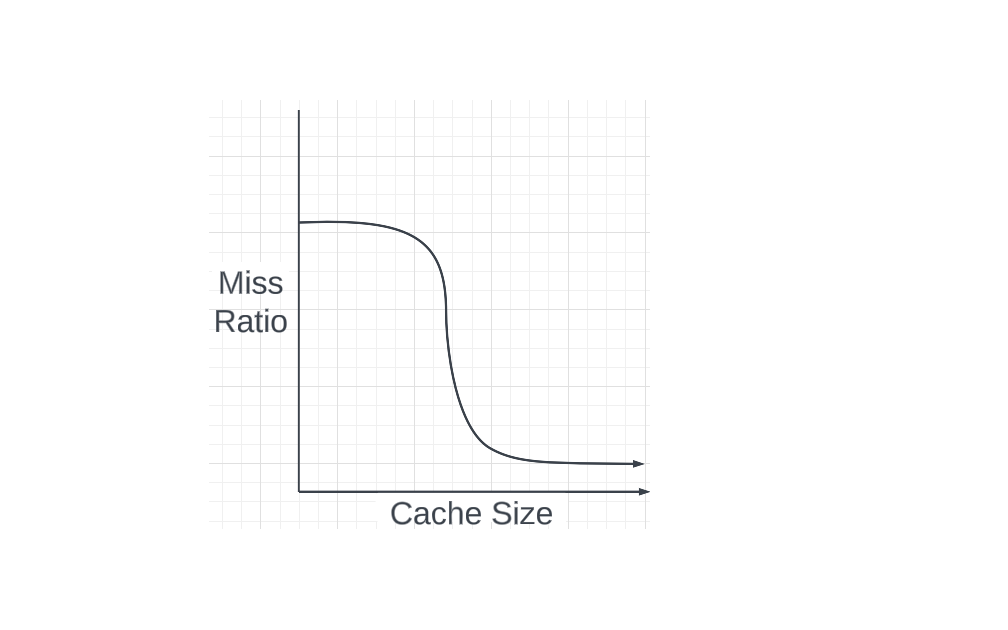
\includegraphics[scale=0.5, trim={.2cm 2.6cm 2.1cm 2.4cm},clip]{thesistemplate_2020-04-24/chapters/MRC shit/mrcFinal.png}
    \caption{Generic MRC}
    \label{fig:my_label}
\end{figure}

Figure 4.1 shows a generalization of what MRCs look like. If a section of the cost curve is almost flat, the cache size is either too large, meaning it misses too little and isn't an efficient use of space, or is too small and isn't gaining the system any efficiency as it misses too often. When designers are creating a cache for a system, they look at this curve and attempt to balance the cost and size to create a cache that improves the system without creating an unnecessary layer of memory.


The naive way to generate these MRCs is to simulate a trace $\sigma$ on all cache sizes with a given algorithm. This requires a large amount of computational effort, as most algorithms when having differing cache sizes make separate choices as to what to evict. An improvement on this method is to only simulate a subset of all cache sizes, but this too is still computationally expensive. There is an important exception to this computationally heavy generation of MRCs, which is to use an algorithm created by \cite{mattson1970evaluation} which allows the generation of an MRC with one pass of the trace $\sigma$.

\section{Mattson's Algorithm}

As stated, the generation of MRCs through running an algorithm on all cache sizes is computationally expensive. Instead, we use an algorithm invented by \cite{mattson1970evaluation} which allows for this generation of MRCs using only $O(nm)$ time where $n$ is the trace length and $m$ is the number of items. Shown here is Mattson's algorithm for LRU in the paging model.


\begin{algorithm}
    \caption{Mattson for LRU}\label{euclid}
        \begin{algorithmic}[1]
            \State $trace = \{i_0 ... i_n \}$
            \For{$x \text{ in range}(0,n) $}
                \State $last\_ Reference = \infty$ \Comment{If an item hasn't been seen before it has $\infty$ priority}
                \For{$z \text{ in range}(x,0) \text{ We go backward in the trace} $}
                    \If {$trace[z] ==trace[x]$} \Comment{trace[x] refers to the item requested}
                        \State $last\_ Reference = z$ \Comment{Update as we have seen the item }
                        \State $\text{Leave Loop}$
                    \EndIf
                \EndFor
                \State $unique\_ Items = \{\}$
                \If{$last\_ Reference \neq \infty$}
                \For{$b \text{ in range}(last\_ Reference,x) $}
                    \If {$trace[b] \text{ not in } unique\_ Items$}
                        \State $\text{push } trace[b] \text{ onto }unique\_ Items$
                    \EndIf
                \EndFor
                \State $Distance = \text{number of items in } unique\_ Items$
                \For{$a \text{ in range}(1,Distance) $}
                    \State $\text{Cost Paid by $cache(a)$}  += cost(trace[x])$ \Comment{cache of size a}
                \EndFor
                \Else 
                    \State $\text{Cost Paid by all cache sizes }  += cost(trace[x])$
                \EndIf
            \EndFor
        \end{algorithmic}
\end{algorithm}

%You don't mention distinctness when you calculate distance, and even if you did, that would still be LRU's stack distance. It's not even accurate for SCP.

When an item $i$ is requested, the number of unique items since the last access is calculated, which is called distance. This distance tells us that all caches with sizes greater than or equal to this number hit on this item as they contain the item in their cache due to LRUs structure. Then all caches with a size less than this number miss on this item and pay its cost as they are too small to still contain the item. In other caching models, when calculating if an item would still be in the cache, you must factor in the size of unique items between repeat requests to the same item, not just the distance in the trace of these requests. 

Here is a generalized version of Mattsons Algorithm
%
\begin{algorithm}
    \caption{Generalized Mattson's for any algorithm}\label{euclid}
        \begin{algorithmic}[1]
            \State $trace = \{i_0 ... i_n \}$
            \State $unique\_ Item\_ Priorities = \{\}$
            \State $unique\_ Items = \{\}$
            \For{$x \text{ in range}(0,n) $}\Comment{trace[x] refers to the item}
                \State $priority = \text{Priority the algorithm assigns to item $trace[x]$ when it is requested}$
                \If {$trace[x] \text{ not in } unique\_ Items$}
                    \State $\text{push } [trace[x],priority] \text{ onto }unique\_ Item\_ Priorities$
                     \State $\text{push } trace[x] \text{ onto }unique\_ Items$
                     \State $\text{Cost Paid by all caches } += cost(trace[x])$
                \Else 
                    \State $size\_Items = 0$
                    \For{$d$ in range $(0,$ (items in $unique\_Item\_ Priorities)$)}
                        \State $size\_ Items+= size(unique\_Item\_ Priorities[d][0])$ \Comment{[d][0] is an item}
                        \If{$unique\_Item\_ Priorities[d][0] == trace[x]$}
                            \State $\text{Cost Paid by all caches of size $<$ $size\_ Items$ } += cost(trace[x])$
                            \State $unique\_Item\_ Priorities[d][1] = priority$             \Comment{update trace[x] priority}
                        \EndIf
                    \EndFor
                \EndIf
                \For{$c \text{ in } unique\_ Item \_Priorities$}
                    \State $currentPriority = c[1]$ \Comment{Which is the current Priority of item c[0]} 
                    \State $change\_ In\_ Priority = 0$             \Comment{An algorithm can choose to alter priority}
                    \If{$\text{request }trace[x]\text{ causes priority change }$}
                        \State $priorityChange =\text{ Priority change of item $c[0]$ from request $trace[x]$}$
                    \EndIf
                    \State $c[1] = currentPriority - newPriority$
                \EndFor
                \State $\text{Reorder $unique\_ Item\_ Priorities$ so item's ordering}$
                \State$\text{in $unique\_ Item\_ Priorities$ goes from highest to lowest priority}$
            \EndFor
        \end{algorithmic}
\end{algorithm}



\begin{algorithm}
    \caption{Generalized Mattson's for any algorithm}\label{euclid}
        \begin{algorithmic}[1]
\State Starting at the beginning of the trace, read the item requests in order and create a priority list of items that starts empty. 
\State For each request, ensure the list is ordered from the item with the highest priority to the item with the lowest priority. 
\State If the item being requested isn't in the priority list, add it to the list with the priority the algorithm assigns and increase the cost paid by all cache sizes by the cost of the item being requested, and move to the next request 
\State Otherwise the item is in the list. Starting from the priority list's beginning, locate the position of the item being requested. As you search for the item, add up the sizes of all items encountered until you find the item being requested. Call this total size d. Then increase the cost paid by all caches of sizes less than d then move to the next request.
\end{algorithmic}
\end{algorithm}


Using this generalized version, you can see that Mattsons algorithm keeps a priority list of all items which is ordered from highest to lowest priority. If an item isn't in this list, all caches must miss and pay its cost. If an item is then in this list, the size of items with priorities greater than the current request's priority is calculated. For all caches that have a size less than this number, they miss and must pay a cost. Then the priorities of all items are updated and reordered, an important note is that some algorithms may not change the priority of an item. This happens in LRU when there are repeated requests to a unique item between requests to the current item, so the item's priorities aren't updated.  
This updating scheme then allows 1 pass of a trace to check all size caches as each request allows the updating of all cache's paid costs. This approach requires that it is limited to a subset of caching algorithms called stack algorithms. 

\subsection{Stack Algorithms}

Stack algorithms are a class of algorithms where: $cache(k) \subseteq cache(k+1)$. This means that all items in $cache(k)$ exist in $cache(k+1)$. This is important as most caching algorithms don't have this structure, this is because their decisions as to what to evict often depend on the size of the cache and the items inside it.

%use diagrams
\begin{figure}[h!]
    \centering
    \caption{How stack algorithms work with differing cache sizes}
    \label{fig:my_label}
\begin{tikzpicture}
 \node[rectangle,draw,  minimum width = 2.9cm, 
    minimum height = 1.1cm, label=above:K-1] (r) at (0,0) {
    };
    \node[rectangle,draw,  minimum width = 3.8cm, 
    minimum height = 2.3cm, label=above:K] (t) at (.4,0) {
    };
    \node[rectangle,draw,  minimum width = 4.8cm, 
    minimum height = 3.3cm, label=above:K+1] (u) at (.9,0) {
    };
    \node[rectangle,draw,  minimum width = 6.2cm, 
    minimum height = 4.5cm, label=above:K+2] (p) at (1.6,0) {
    };
\node[rectangle,draw, minimum width = 4cm, 
    minimum height = 1cm,below right = -0.5cm and -1.5cm of r] (q) at (0,0) {
    \begin{tikzpicture}
            \node[rounded corners,draw=black,minimum size=0.8cm]{a};
    \end{tikzpicture}
    \begin{tikzpicture}
        \node[rounded corners,draw=black,minimum size=0.8cm]{b};
    \end{tikzpicture}
    \begin{tikzpicture}
        \node[rounded corners,draw=black,minimum size=0.8cm]{d};
    \end{tikzpicture}
    \begin{tikzpicture}
        \node[rounded corners,draw=black, minimum size=0.8cm]{e};
    \end{tikzpicture}
    \begin{tikzpicture}
            \node[rounded corners,draw=black,minimum size=0.8cm]{f};
    \end{tikzpicture}
    \begin{tikzpicture}
        \node[rounded corners,draw=black,minimum size=0.8cm]{g};
    \end{tikzpicture}
    };
\end{tikzpicture}
\end{figure}
%\begin{figure}
    \centering
    \caption{Size k=3 cache vs k=4 cache in stack algorithm }
    \label{fig:my_label}
\begin{tikzpicture}


    \node[rounded corners,draw=black,label=above:K, minimum size=2cm] (a) at (0,0)  {
    \begin{tikzpicture}
        \node[rounded corners,draw=black,minimum size=0.8cm]{a};
    \end{tikzpicture}
    \begin{tikzpicture}
        \node[rounded corners,draw=black,minimum size=0.8cm]{};
    \end{tikzpicture}
    \begin{tikzpicture}
        \node[rounded corners,draw=black,minimum size=0.8cm]{};
    \end{tikzpicture}
    };
    \node[text width=3cm] at (-3, 0) 
    {Cold start miss, a added to cache};

    
    \node[rounded corners,draw=black,minimum size=2cm] (b) at (0,-2.5)  {   \begin{tikzpicture}
        \node[rounded corners,draw=black,minimum size=0.8cm]{a};
    \end{tikzpicture}
    \begin{tikzpicture}
        \node[rounded corners,draw=black,minimum size=0.8cm]{b};
    \end{tikzpicture}
    \begin{tikzpicture}
        \node[rounded corners,draw=black,minimum size=0.8cm]{};
    \end{tikzpicture}
    };
     \node[text width=3cm] at (-3,-2.5) 
    {Cold start miss, b added to cache};

    
    \node[rounded corners,draw=black,minimum size=2cm] (c) at (0,-5)  {   \begin{tikzpicture}
        \node[rounded corners,draw=black,minimum size=0.8cm]{a};
    \end{tikzpicture}
    \begin{tikzpicture}
        \node[rounded corners,draw=black,minimum size=0.8cm]{b};
    \end{tikzpicture}
    \begin{tikzpicture}
        \node[rounded corners,draw=black,minimum size=0.8cm]{c};
    \end{tikzpicture}
    };
    \node[text width=3cm] at (-3,-5) 
    {Cold start miss, c added to cache};

      
    \node[rounded corners,draw=black,minimum size=2cm] (d) at (0,-7.5)  {   \begin{tikzpicture}
        \node[rounded corners,draw=black,minimum size=0.8cm]{a};
    \end{tikzpicture}
    \begin{tikzpicture}
        \node[rounded corners,draw=black,minimum size=0.8cm]{b};
    \end{tikzpicture}
    \begin{tikzpicture}
        \node[rounded corners,draw=black,minimum size=0.8cm]{d};
    \end{tikzpicture}
    };

     \node[text width=3cm] at (-3,-7.5) 
    {Cold start miss, D added to cache, evict C since FITF};

    
    \node[rounded corners,draw=black,minimum size=2cm, below left=1 cm of d] (e) at (2.2,-8.4)  { 
    \begin{tikzpicture}
        \node[rounded corners,draw=black,minimum size=0.8cm]{a};
    \end{tikzpicture}
    \begin{tikzpicture}
        \node[rounded corners,draw=black,minimum size=0.8cm]{b};
    \end{tikzpicture}
    \begin{tikzpicture}
        \node[rounded corners,draw=black,minimum size=0.8cm]{d};
    \end{tikzpicture}
    };  

     \node[text width=3cm] at (-2.5,-9.8) 
    {Hit on A};
    
    \node[rounded corners,draw=black,minimum size=2cm,below left=1 cm of e] (f) at (2.2,-10.8)  { 
    \begin{tikzpicture}
        \node[rounded corners,draw=black,minimum size=0.8cm]{a};
    \end{tikzpicture}
    \begin{tikzpicture}
        \node[rounded corners,draw=black,minimum size=0.8cm]{b};
    \end{tikzpicture}
    \begin{tikzpicture}
        \node[rounded corners,draw=black,minimum size=0.8cm]{d};
    \end{tikzpicture}
    };  

     \node[text width=3cm] at (-2.5,-12.2) 
    {Hit on B};

    
    \node[rounded corners,draw=black,minimum size=2cm, below left=1 cm of f] (g) at (2.2,-13.4)  { 
    \begin{tikzpicture}
        \node[rounded corners,draw=black,minimum size=0.8cm]{a};
    \end{tikzpicture}
    \begin{tikzpicture}
        \node[rounded corners,draw=black,minimum size=0.8cm]{b};
    \end{tikzpicture}
    \begin{tikzpicture}
        \node[rounded corners,draw=black,minimum size=0.8cm]{d};
    \end{tikzpicture}
    };  

     \node[text width=3cm] at (-3,-14.7) 
    {Capacity miss C, evict D};
    
    \node[rounded corners,draw=black,minimum size=2cm, below left=1 cm of g] (h) at (2.2,-15.6)  { 
    \begin{tikzpicture}
        \node[rounded corners,draw=black,minimum size=0.8cm]{a};
    \end{tikzpicture}
    \begin{tikzpicture}
        \node[rounded corners,draw=black,minimum size=0.8cm]{b};
    \end{tikzpicture}
    \begin{tikzpicture}
        \node[rounded corners,draw=black,minimum size=0.8cm]{c};
    \end{tikzpicture}
    }; 
    \node[text width=3cm] at (-2.5,-17.3) 
    {Hit on C};
     \node[rounded corners,draw=black,label=above:k+1, minimum size=2cm] (i) at (6,0)  {
    \begin{tikzpicture}
        \node[rounded corners,draw=black,minimum size=0.8cm]{};
    \end{tikzpicture}
    \begin{tikzpicture}
        \node[rounded corners,draw=black,minimum size=0.8cm]{};
    \end{tikzpicture}
    \begin{tikzpicture}
        \node[rounded corners,draw=black,minimum size=0.8cm]{};
    \end{tikzpicture}
    \begin{tikzpicture}
        \node[rounded corners,draw=black,minimum size=0.8cm]{d};
    \end{tikzpicture}
    };
    
    \node[rounded corners,draw=black,minimum size=2cm] (j) at (6,-2.5)  {   \begin{tikzpicture}
        \node[rounded corners,draw=black,minimum size=0.8cm]{a};
    \end{tikzpicture}
    \begin{tikzpicture}
        \node[rounded corners,draw=black,minimum size=0.8cm]{};
    \end{tikzpicture}
    \begin{tikzpicture}
        \node[rounded corners,draw=black,minimum size=0.8cm]{};
    \end{tikzpicture}
    \begin{tikzpicture}
        \node[rounded corners,draw=black,minimum size=0.8cm]{d};
    \end{tikzpicture}
    };
    
    \node[rounded corners,draw=black,minimum size=2cm] (k) at (6,-5)  {   \begin{tikzpicture}
        \node[rounded corners,draw=black,minimum size=0.8cm]{a};
    \end{tikzpicture}
    \begin{tikzpicture}
        \node[rounded corners,draw=black,minimum size=0.8cm]{b};
    \end{tikzpicture}
    \begin{tikzpicture}
        \node[rounded corners,draw=black,minimum size=0.8cm]{};
    \end{tikzpicture}
    \begin{tikzpicture}
        \node[rounded corners,draw=black,minimum size=0.8cm]{d};
    \end{tikzpicture}
    };

      
    \node[rounded corners,draw=black,minimum size=2cm] (l) at (6,-7.5)  {   \begin{tikzpicture}
        \node[rounded corners,draw=black,minimum size=0.8cm]{a};
    \end{tikzpicture}
    \begin{tikzpicture}
        \node[rounded corners,draw=black,minimum size=0.8cm]{b};
    \end{tikzpicture}
    \begin{tikzpicture}
        \node[rounded corners,draw=black,minimum size=0.8cm]{c};
    \end{tikzpicture}
    \begin{tikzpicture}
        \node[rounded corners,draw=black,minimum size=0.8cm]{d};
    \end{tikzpicture}
    };
    
    \node[rounded corners,draw=black,minimum size=2cm, below left=1 cm of l] (m) at (8.7,-8.4)  { 
    \begin{tikzpicture}
        \node[rounded corners,draw=black,minimum size=0.8cm]{a};
    \end{tikzpicture}
    \begin{tikzpicture}
        \node[rounded corners,draw=black,minimum size=0.8cm]{??};
    \end{tikzpicture}
    \begin{tikzpicture}
        \node[rounded corners,draw=black,minimum size=0.8cm]{d};
    \end{tikzpicture}
    \begin{tikzpicture}
        \node[rounded corners,draw=black,minimum size=0.8cm]{d};
    \end{tikzpicture}
    };  
    \node[rounded corners,draw=black,minimum size=2cm,below left=1 cm of m] (n) at (8.7,-10.8)  { 
    \begin{tikzpicture}
        \node[rounded corners,draw=black,minimum size=0.8cm]{a};
    \end{tikzpicture}
    \begin{tikzpicture}
        \node[rounded corners,draw=black,minimum size=0.8cm]{b};
    \end{tikzpicture}
    \begin{tikzpicture}
        \node[rounded corners,draw=black,minimum size=0.8cm]{d};
    \end{tikzpicture}
    \begin{tikzpicture}
        \node[rounded corners,draw=black,minimum size=0.8cm]{d};
    \end{tikzpicture}
    };  
    \node[rounded corners,draw=black,minimum size=2cm, below left=1 cm of n] (o) at (8.7,-13.4)  { 
    \begin{tikzpicture}
        \node[rounded corners,draw=black,minimum size=0.8cm]{a};
    \end{tikzpicture}
    \begin{tikzpicture}
        \node[rounded corners,draw=black,minimum size=0.8cm]{b};
    \end{tikzpicture}
    \begin{tikzpicture}
        \node[rounded corners,draw=black,minimum size=0.8cm]{d};
    \end{tikzpicture}
    \begin{tikzpicture}
        \node[rounded corners,draw=black,minimum size=0.8cm]{d};
    \end{tikzpicture}
    };  
    \node[rounded corners,draw=black,minimum size=2cm, below left=1 cm of o] (p) at (8.7,-15.9)  { 
    \begin{tikzpicture}
        \node[rounded corners,draw=black,minimum size=0.8cm]{a};
    \end{tikzpicture}
    \begin{tikzpicture}
        \node[rounded corners,draw=black,minimum size=0.8cm]{b};
    \end{tikzpicture}
    \begin{tikzpicture}
        \node[rounded corners,draw=black,minimum size=0.8cm]{d};
    \end{tikzpicture}
    \begin{tikzpicture}
        \node[rounded corners,draw=black,minimum size=0.8cm]{d};
    \end{tikzpicture}
    };  
                
    \draw[thick,->] (i) -- (j);
    \draw[thick,->](j) -- (k);  
    \draw[thick,->](k) -- (l);  
    \draw[thick,->](l) -- (m);  
    \draw[thick,->] (m) -- (n);
    \draw[thick,->](n) -- (o);  
    \draw[thick,->](o) -- (p);
\end{tikzpicture}
\end{figure}

Figure 4.2 shows a stack algorithm's cache states. As can be seen $\forall x < k, \text{ } cache(x) \subseteq cache(k)$. Showing an algorithm follows this rule on any trace is sufficient to prove it is a stack algorithm.  

%talk about this being the ordering of items, requesting particular items, this thing called stack distance
Looking back to LRU in Chapter 3, we show here that it is a stack algorithm. The proof for this is quite simple, as LRUs structure is based upon the item's last reference from the current request in the trace. So cache(k) $\subseteq$ cache(k+1) as
%\newtheorem{theorem}{Theorem}[section]
\newtheorem{corollary}{Corollary}[theorem]
\newtheorem{lemma}[theorem]{Lemma}
\newtheorem{definition}{Definition}[section]
\begin{lemma}
    LRUs $cache(k) \subseteq cache(k+1)$
\end{lemma}
LRU always evicts $f_{minPriority} \in cache(LRU)$ when item $i_n$ is requested and cache(LRU) can't contain size($i_n$). Now looking at cache(k+1) after request $i_n$, we know that 

\[cache(k+1) = \{i_{n-(k+1)},..., i_n \} \]
then look at cache k after request $i_n$
\[cache(k) = \{i_{(n-k)},..., i_{n} \} \]

Then, at request $i_n$
\[cache(k) \subseteq cache(k+1)\]

Using \ref{pythagorean} when cache(k) received request $i_{n-1}$ it evicted $i_{n-(k+2)}$ while cache(k+1) evicted $i_{n-(k+1)}$. This shows that  
\[\forall i_n, \textbf{ } cache(k) \subseteq cache(k+1) \]
$\qed$
when needing to evict an element, $cache(k)$ evicts the $k+1$ least referenced item, which is quite obviously still in $cache(k+1)$.


When looking at a trace of items for LRU, such as in Figure 4.2, it is important to note the number of items between requests for the same unique item. This number is called the stack distance and is what Mattson's algorithm uses to decide if an item is a hit or miss on a specific cache size for LRU. When this distance is greater than the size of the cache, the request causes a miss, but if the distance is less than the size of the cache the request is a hit. For algorithms other than LRU, this distance that Mattson's algorithm uses is a number of items in higher priority order, not the number of unique items between requests.

Now that there is the context for why Mattson's algorithm functions to generate an MRC, here is an example of how it manages to correctly show the cost for LRU on a trace.
\begin{figure}[H]
    \centering
    \caption{LRU priority queue of elements on the trace: A,B,C,B,A,D,C}
    \label{fig:my_label}
\newcounter{row}
\newcounter{col}

\newcommand\setrow[9]{
  \setcounter{col}{-3}
  \foreach \n in {#1, #2, #3, #4, #5, #6, #7, #8, #9} {
    \edef\x{\value{col} - 0.4}
    \edef\y{5.5 - \value{row}}
    \node[anchor=center] at (\x, \y) {\n};
    \stepcounter{col}
  }
  \stepcounter{row}
}

\newcommand\setrows[9]{
  \setcounter{col}{-1}
  \foreach \n in {#1, #2, #3, #4, #5, #6, #7, #8, #9} {
    \edef\x{\value{col} - 0.4}
    \edef\y{5.5 - \value{row}}
    \node[anchor=center] at (\x, \y) {\n};
    \stepcounter{col}
  }
  \stepcounter{row}
}
\begin{tikzpicture}[scale=1]

\begin{scope}
\draw (0, 0) grid (7, 4);
\draw[very thin] (0, 0) grid (7, 4);
\draw[thick,-] (1,1) -- (4,1);
\draw[thick,-] (1,1) -- (1,4);
\draw[thick](1,4) --(4,4);
\draw[thick](4,1) --(4,4);
\setcounter{row}{1}
\setrow {}{\textbf{Requests:}}{}{A}{B}{C}{B}{A}{D}
\setrow {\textbf{Priority}}{}{High}{}{A}{B}{C}{B}{A}
\setrow {}{}{$\downarrow$}{ }{}{}{}{}{}
\setrow {}{}{$\downarrow$}{ }{}{}{}{}{}
\setrow {}{}{Low}{}{}{}{}{}{}

\end{scope}
\begin{scope}
\setcounter{row}{1}
\setrows {}{}{}{}{}{}{}{C}{}
\setrows {}{}{}{}{}{}{A}{D}{C}
\setrows {}{}{}{A}{B}{C}{B}{A}{D}
\setrows {}{}{}{}{A}{A}{C}{B}{A}
\setrows {}{}{}{}{}{}{}{C}{B}
\end{scope}
\end{tikzpicture}
\end{figure}
Figure 4.3 shows the priority of elements in an LRU cache on a trace. This priority queue is mimicked by Mattson's algorithm as the queue position of the item in its stack distance.
\begin{figure}[H]
    \centering
    \caption{the priority of items after request to D}
    \label{fig:my_label}
\newcounter{row2}
\newcounter{col2}

\newcommand\setrows[4]{
  \setcounter{col2}{1}
  \foreach \n in {#1, #2, #3, #4} {
    \edef\x{\value{col2} - 0.5}
    \edef\y{7.5 - \value{row2}}
    \node[anchor=center] at (\x, \y) {\n};
    \stepcounter{col2}
  }
  \stepcounter{row2}
}
\begin{tikzpicture}[scale=1]

\begin{scope}
\draw (0, 0) grid (4, 1);
\draw[very thin] (0, 0) grid (4, 1);
\setcounter{row2}{7}
\setrows{D}{A}{B}{C}
\end{scope}
\end{tikzpicture}
\\
and compare it to the caches of sizes 3 and 4
\\
\begin{tikzpicture}
        \node[rounded corners,draw=black,minimum size=2cm, label=above: cache size 4] (o) at (0,0)  { 
    \begin{tikzpicture}
        \node[rounded corners,draw=black,minimum size=0.8cm]{A};
    \end{tikzpicture}
    \begin{tikzpicture}
        \node[rounded corners,draw=black,minimum size=0.8cm]{B};
    \end{tikzpicture}
    \begin{tikzpicture}
        \node[rounded corners,draw=black,minimum size=0.8cm]{D};
    \end{tikzpicture}
    \begin{tikzpicture}
        \node[rounded corners,draw=black,minimum size=0.8cm]{C};
    \end{tikzpicture}
    };  
        \node[rounded corners,draw=black,minimum size=2cm,label=above: cache size 3] (o) at (5,0)  { 
    \begin{tikzpicture}
        \node[rounded corners,draw=black,minimum size=0.8cm]{A};
    \end{tikzpicture}
    \begin{tikzpicture}
        \node[rounded corners,draw=black,minimum size=0.8cm]{B};
    \end{tikzpicture}
    \begin{tikzpicture}
        \node[rounded corners,draw=black,minimum size=0.8cm]{D};
    \end{tikzpicture}
    };  
\end{tikzpicture}
\end{figure}


As can be seen in Figure 4.4, $C$ is requested at timestep 2, and then again at timestep 6. After timestep 6 $C \in cache(4)$ but was evicted to make room for $D$ in a $cache(3)$. This example then shows how LRU assigns its item priorities based on distance from the last request and how Mattson's algorithm manages to get the correct costs for these caches.

An important thing to note is that the priority stemming from distance since the 
last request is how LRU maintains its priority list. Stack algorithms don't necessarily have to organize their priority from the stack distance itself, instead, the priorities can be some function of cost, size, or distance.